%!TEX root = thesis.tex
\chapter{Einleitung}
\label{cha:einleitung}
Die Konzepte der Nanotechnologie haben die Grenzen der herkömmlichen Technologie überschritten und neue Horizonte der Wissenschaft und Technik eröffnet. Unter diesen Konzepten befindet sich das \emph{Nanonetzwerk}, ein innovatives Netzwerk, das aus einer Sammlung von Nanomaschinen besteht, die miteinander interagieren und kommunizieren können. In diesem Kapitel soll eine Motivation für das Thema, der wissenschaftliche Beitrag dieser Arbeit und die Struktur der Arbeit vorgestellt werden.

\section{Motivation/Problemstellung}

Nanonetzwerke öffnen ein neues Fenster in die Welt der Mikro- und Nanotechnologie und zeigen großes Potenzial für Anwendungen in der Medizin, Umweltüberwachung, Materialwissenschaft und einigen anderen Bereichen \cite{akyildiz2011nano}. Sie ermöglichen die Kommunikation und den Informationsaustausch auf der Nanoskala, was einen grundlegend neuen Ansatz für die Kommunikation und den Informationsaustausch darstellt. Wie klein die Nanoebene ist, ist für einige Personen schwer einzuschätzen. Ein typischer Vergleich dafür ist die Breite eines Haares. Ein Haar ist je nach Beschaffenheit 0,05 bis 0,08 Millimeter breit. Das sind umgerechnet 50.000 bis 80.000 Nanometer. Vergleichsweise dazu beträgt die Breite eines DNA-Strangs 2,5 Nanometer \cite{wiki2023haar, wiki2023dna}. Diese Skala führt zu einer neuen Dimension von Netzwerken, die über die bisher bekannten Grenzen hinausgehen.

\begin{figure}
	\includegraphics[width=\textwidth]{images/nanomachines.png}
	\caption[Nanotechnologien Unterscheidungen]{Biologische und menschengemachte Strukturen, die entweder durch ein Top-Down oder Bottom-Up Ansatz für Nanotechnologien verwendet werden können.\cite{akyildiz2011nano}}
	\label{fig:nanomachines}
\end{figure}

Nanotechnologien können eine Vielzahl von Strukturen und Partikeln umfassen, die sich in Funktion und Fähigkeiten erheblich unterscheiden können. Je nach Anwendung können verschiedene Strukturen verwendet werden, was zur Vielseitigkeit dieser Technologie beiträgt. Einige Beispiele dieser Strukturen sind in Abbildung~\ref{fig:nanomachines} zu sehen.

Es ist zu beachten, dass in der Welt der Nanotechnologien eine Unterscheidung zwischen biologischen und menschengemachten Materialien gemacht wird. Biologische Nanomaschinen nutzen biologische Mechanismen und Prozesse, während menschengemachte Maschinen auf künstlichen Materialien und Herstellungsprozessen basieren.

Diese Arbeit konzentriert sich auf eine spezielle Art von Nanonetzwerken: auf die DNA-basierten Nanonetzwerke. Diese verwenden die Struktur und die Eigenschaften von DNA-Molekülen, um Netzwerke zu bilden und Funktionen auszuführen. Im weiteren Verlauf dieser Arbeit wird der Begriff \glqq Nanonetzwerke\grqq~speziell auf diese Art von Netzwerken bezogen, es sei denn, es wird anders angegeben.

Die Bedeutung von DNA-basierten Nanonetzwerken kann nicht hoch genug eingeschätzt werden, da sie eine breite Palette von Anwendungen ermöglichen, von der gezielten Medikamentenabgabe bis zur Biosensorik und darüber hinaus. Indem das Verständnis und die Fähigkeiten in diesem Bereich erweitert werden, öffnen sich die Türen zu revolutionären Fortschritten in einer Vielzahl von Disziplinen.

\begin{figure}
	\centering 
	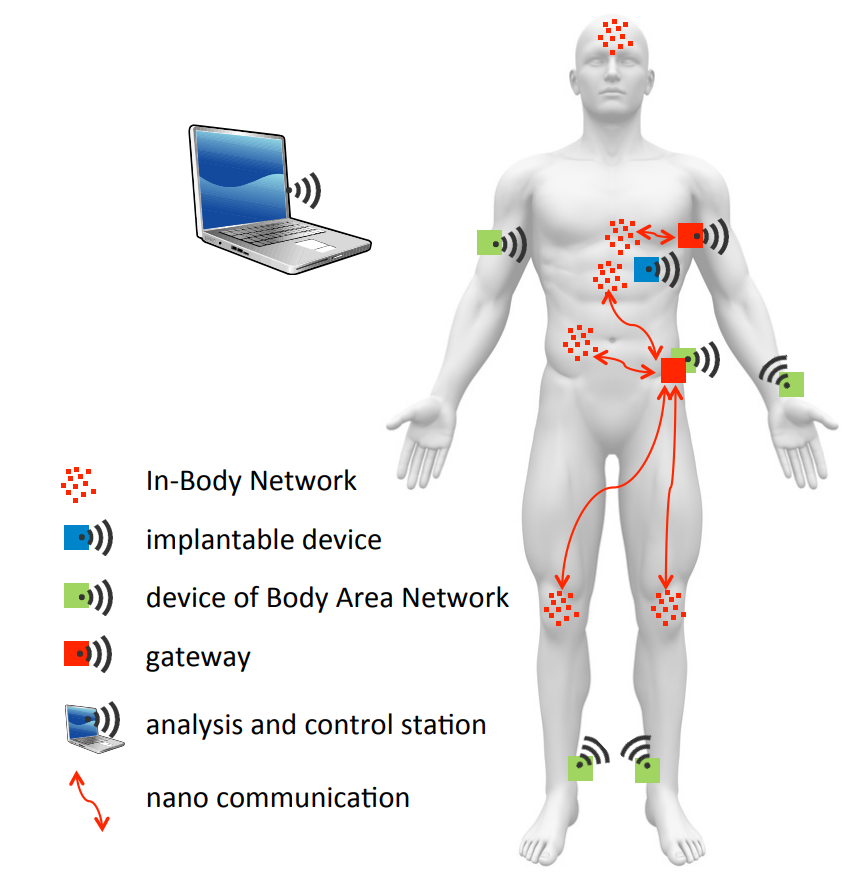
\includegraphics[width=0.53\textwidth]{images/In-Body_Networks.png}
	\caption[In-Body-Netzwerke]{In-Body-Netzwerke kombiniert mit einem Body-Area-Network (BAN). Eine Kontrollstation, welche für die Analyse von Daten zuständig ist, kommuniziert über drahtlose Verbindungen mit im Körper implantierten Geräten. Diese Geräte können wiederum miteinander oder über ein Gateway mit In-Body-Networks kommunizieren.\cite{dressler2015nanothings}}
	\label{fig:in-body_network}
\end{figure}

Wie zuvor angedeutet, gibt es einige verschiedene Anwendungsgebiete für Nanotechnologien und im Besonderen für Nanonetzwerke.
Das größte und möglicherweise wichtigste Anwendungsgebiet ist jedoch die Medizin \cite{gu2013diabetes,li2018nanorobo,wang2015light,yao2017factors}.
Nanopartikel im Spezifischen werden beispielsweise schon länger zur Krebsbekämpfung eingesetzt \cite{singhal2010cancer}.

Es lassen sich auch andere mögliche Anwendungsgebiete für diese Technologie finden, wie beispielsweise in der Geologie \cite{jin2019mapping}, in der Agrartechnik \cite{almpanis2019agent,axelos2017agri} oder in der Materialindustrie \cite{ma2010qca,taibi2019light}. Doch die Fähigkeit von Nanonetzwerken, auf einem deutlich kleineren Skalenbereich als herkömmliche Netzwerke zu agieren, verleiht ihnen ein hohes Potenzial für Anwendungen im Bereich der Humanmedizin.

Zwar werden einige diese Technologien heute schon verwendet, doch das Potenzial ist noch lange nicht voll ausgeschöpft.
So können diese bereits implementierten Technologien in ein \emph{In-Body-Network} (IBN) zusammengefügt werden.
Das theoretische Nanonetzwerk funktioniert mit einer Kontrollstation, die mit Geräten verbunden ist, die beispielsweise unter der Haut eines Menschen implantiert werden können.
Diese Geräte werden wiederum dafür verwendet, um über den menschlichen Blutkreislauf miteinander und mit der externen Kontrollstation zu kommunizieren.
Ein solches System kann nicht nur die Vitalwerte des Körpers überwachen, sondern diese Daten zur Analyse und Auswertung an die Kontrollstation geben.
Wiederum kann die Kontrollstation anhand der ausgewerteten Daten Anweisungen an das In-Body-Network senden, das daraufhin entsprechende Medikamente an spezifischen Stellen des Körpers anwenden kann.
Ein solches Netzwerk, wie es in Abbildung~\ref{fig:in-body_network} dargestellt ist, kann mit heutigem Stand zwar noch nicht \emph{in-vivo} (im lebendigen Organismus) realisiert werden, doch die theoretischen Modelle sind schon so weit, dass sie auf mathematischer Ebene funktionsfähig sind.

Jedoch gibt es bislang keine konkreten Ansätze, um die kleinschrittige Kommunikation mit DNA-Tiles und ihrer Self-Assembly zu regeln. Wie kann Information in Self-Assemblies abgebildet werden? Welche Mechanismen aus herkömmlichen Kommunikationsprotokollen lassen sich auf einer so kleinen Ebene übersetzen? Wie funktioniert Adressierung oder Fehlererkennung in einer Self-Assembly? Diese und andere Fragen haben dazu geführt, dass diese Arbeit sich kleinschrittiger und tiefer mit diesem Thema der Nanonetzwerke befasst.

\section{Der wissenschaftliche Beitrag dieser Arbeit}
Diese Arbeit soll eine umfangreiche Grundlage für die Kommunikation mit DNA-Tile-basierten Self-Assemblies schaffen. Die Ansätze und Ideen sollen dementsprechend möglichst allgemein gehalten werden, sodass sie für verschiedene Anwendungsgebiete angepasst werden können. Auch soll mit dieser Arbeit ein Gefühl übermittelt werden, welche Mechanismen herkömmlicher Kommunikationsprotokolle mit Tile-basierter Self-Assembly implementierbar sind und welche nicht. Leser*innen dieser Arbeit sollen am Ende Inspiration und Gedankenanstöße für eigene Forschung auf dem Gebiet erhalten.

\section{Struktur der Arbeit}
Die Arbeit ist in sieben Kapitel unterteilt. Nach der Einleitung in diesem Kapitel folgen mit Kapitel~\ref{cha:grundlagen} die Grundlagen für DNA-basierte Nanonetzwerke. In den Grundlagen finden sich Informationen über DNA, verschiedene Tilebildungsverfahren von DNA-Strängen, Self-Assembly der Tiles und Assemblymodelle. Auch werden Grundlagen zu herkömmlichen Kommunikationsprotokollen geliefert. Nach den Grundlagen werden in Kapitel~\ref{cha:relatedwork} wissenschaftliche Arbeiten näher betrachtet, da diese eine besondere Nähe zu dieser Arbeit besitzen.

Nach den Grundlagen werden in Kapitel~\ref{cha:konzept} die Konzepte vorgestellt, die für die Umsetzung von Mechanismen aus herkömmlichen Kommunikationsprotokollen auf Nanoebene notwendig sind. Von Adressierung, Routing, Fehlererkennung, Fehlerkorrektur, Framing, Datenflusskontrolle, Nachrichtencodierung zu Flags, werden verschiedene Ideen modelliert und vorgestellt. Einige dieser Ideen wurden in einem Python Skript \marginnote{\qrcode[height=1cm]{https://github.com/Falkenheim/Tile-Generator}} implementiert, das Tilesets für die Simulationsumgebung NetTAS verändert oder generiert. Das Skript und die Umsetzung der Mechanismen werden in Kapitel~\ref{cha:konstruktion} vorgestellt.

Die betrachteten Tilesets und ihre Simulationsergebnisse werden im Kapitel~\ref{cha:simulationen} analysiert und ausgewertet. In Kapitel~\ref{cha:zusammenfassung} wird abschließend eine Zusammenfassung der Arbeit geliefert.

Da eine Motivation und ein grober Überblick für die Arbeit geliefert wurde, kann mit dem detaillierteren Inhalt der Arbeit begonnen werden.
























%Keine Überschrift ohne Text $\dots$

%\section{Das Lübecker Holstentor}
%\label{sec:holstentor}

%\subsection{Zitieren}
%\label{sec:cite}

%Das Eigenbase-Projekt \cite{Akyildiz2008a} ist sehr cool.

%\subsection{Grafik}

%See also Grafiken in commands.tex ab Zeile 341 für subfigures etc.
%\begin{figure}[htbp]
%	\begin{center}
%		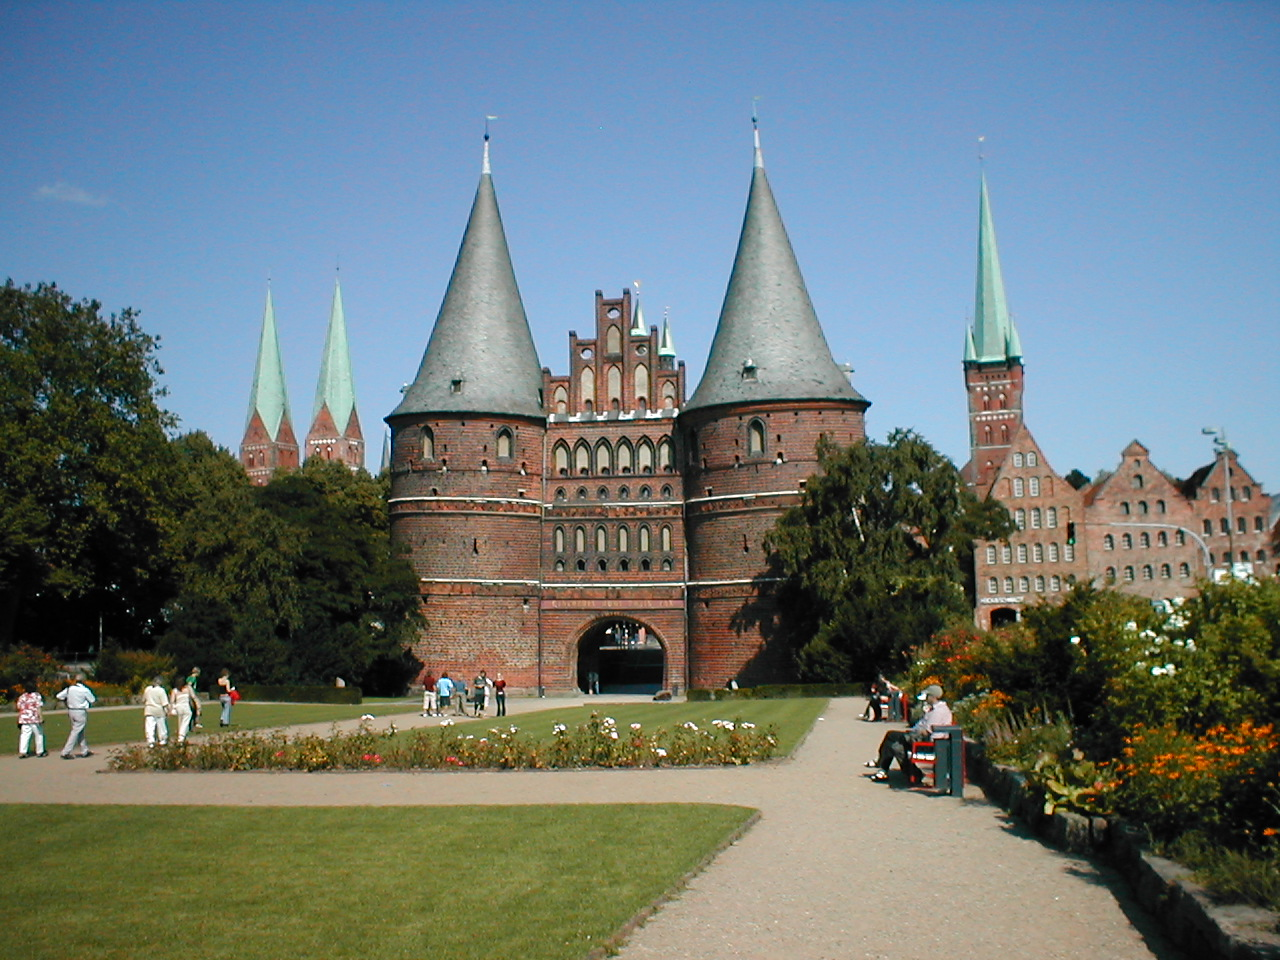
\includegraphics[width=0.75\textwidth]{images/LuebeckHolstentor}
%		\caption[Kurzfassung für Abbildungsverzeichnis]{Ausführlicher Titel}
%		\label{fig:Holstentor}
%		\end{center}
%\end{figure}

%Cref ergänzt automatisch Abbildung oder Tabellle etc.
%In \Cref{fig:Holstentor} sehen wir das \todo{Eine Randnotiz!} Lübecker Holstentor.

%\subsection{Tabelle}

%\begin{table}
%\centering
%\footnotesize
%\caption[Kurze Tabellenüberschrift]{Lange Tabellenüberschrift}
%\label{tab:eins}
%\begin{tabular}{p{1.4cm} p{2.0cm} p{2.0cm}}\toprule
%			& A 			& B 		\\[0.1cm]\midrule
%	1		& w				& s 		\\[0.2cm]
%	2 		& e				& f			\\[0.2cm]
%	3		& r				& s			\\[0.2cm]
%	4 		& t				& n 		\\\bottomrule
%\end{tabular}
%\end{table}

%In \Cref{tab:eins} sehen wir...

%\subsection{Gleichung}

%\begin{equation}\label{eq:test}
%  a=b
%\end{equation}

%In \Cref{eq:test} sehen wir...

%\subsection{Code-Listing}

%\lstinputlisting[label={lst:hello}, caption={This is a code.}]{helloworld.cpp}


%In \Cref{lst:hello} wird...

%\subsection{Zitat}

%Ein Zitat aus der Wikipedia:

%\begin{quote}
%	\begin{myquote}
%		Die Universität zu Lübeck ist eine Hochschule in der Hansestadt Lübeck (Deutschland), die 1964 zunächst als zweite Medizinische Fakultät der Universität Kiel eingerichtet wurde. Studienangebot und Forschungstätigkeit der Universität zu Lübeck haben ihren Ausgangspunkt in der Medizin.
%		\label{quote:uni}
%	\end{myquote}
%\end{quote}

%\todo[inline,color=green!40,caption={Kurzversion des Todos}]{Ein Inline-Todo}

%
% Hinweis: CRef funktioniert nicht für Zitate! Bitte \quoteref{...} verwenden
%
%In \quoteref{uni}...

%\todo[inline]{Mit Besitzer und Datum}

%\newpage

%Etwas mehr Inhalt auf einer weiteren Seite

%\newpage

%Etwas mehr Inhalt auf noch einer tollen Seite
